\documentclass[a4paper,11pt]{article}

\usepackage{fullpage}
\usepackage{color}
\usepackage{hyperref}
\usepackage{amsmath}
\usepackage{amssymb}
\usepackage{tikz}
\usepackage{tabularx}
\usepackage{booktabs}
\usepackage{amsmath}
\usepackage{multirow}
\usepackage{layouts}
\usepackage{array}
\usepackage{pgf}
\usepackage{tikz}
\usepackage{amssymb}
\usepackage{graphics}
\usepackage{eucal}
\usepackage{ifthen}
\usepackage{ifpdf}
\usepackage{lmodern}
\usepackage{amsthm}
\usepackage{epstopdf}
\usetikzlibrary{positioning}

\hypersetup{
  colorlinks,%
    citecolor=black,%
    filecolor=black,%
    linkcolor=black,%
    urlcolor=mygreylink     % can put red here to visualize the links
}

\definecolor{hlcolor}{rgb}{1, 0, 0}
\definecolor{mygrey}{gray}{.85}
\definecolor{mygreylink}{gray}{.30}
\textheight=8.6in
\raggedbottom
\addtolength{\oddsidemargin}{-0.375in}
\addtolength{\evensidemargin}{0.375in}
\addtolength{\textwidth}{0.5in}
\addtolength{\topmargin}{-.375in}
\addtolength{\textheight}{0.75in}

\newcommand{\resheading}[1]{{\large \colorbox{mygrey}{\begin{minipage}{\textwidth}{\textbf{#1 \vphantom{p\^{E}}}}\end{minipage}}}}

\newcommand{\mywebheader}{
  \begin{tabular}{@{}p{5in}p{4in}}
  {\resheading{Assignment 3: Multi Agent Planning and Learning}} & {\Large 21 October, 2012}\\\vspace{0.2cm}
  \end{tabular}}

\begin{document}


\begin{center}
{\LARGE \textbf{Autonomous Agents}}\\ [1em]
\end{center}
\mywebheader

\begin{center}
{\Large By:} \\ \vspace{0.1cm}
{\Large Paris Mavromoustakos} \\  \vspace{0.1cm}
{\Large Georgios Methenitis} \\ \vspace{0.1cm}
{\Large Patrick de Kok} \\ \vspace{0.1cm}
{\Large Marios Tzakris}
\end{center}


\section{Introduction}

In this last assignment, we added multiple predators to the environment, while making the prey intelligent, therefore, harder to catch. Our previous implementations already considered the prey to be an agent, for that reason we only made minor changes to our prey's functions, allowing it to use learning methods just like the predators. The prey will now move with equal probability towards all directions, always, with a chance to trip, it stays in the same position independently from the action that it chooses, otherwise one predator would never be able to catch it.

What we also changed is that the prey and predator(s) move simultaneously, in a single time-step. That means, the agents can be next to each other and swap positions, without considering their next move to be "safe" or not.

Last, we now consider this implementation to be a zero-sum Markov game, because predators are going to receive a negative $-10$ reward if they crash into each other, while the prey will be receiving a positive $+10$ reward. Beside that, the predators will receive reward $+10$ for catching the prey which gets $-10$ for getting caught.



\section{Exercise 1}

In the first exercise, we use the $11 \times 11$ grid where we add a prey and more than one predators. Our implementation requests the number of predators as input from the user, initializes the prey at position $<5,5>$ and puts the predators in random positions. 

The agents then move randomly on the grid until two predators move into the same position (Collision) or a predator catches the prey (Catch). These two are the only possible absorbing states. We should note, that, if two predators collide and the prey is caught in the same time-step, the predators' collision is more "important" and defines the reward distribution.


\subsection{Results}
Table~\ref{table:multirandom}, presents the results we had in the first part of the exercise. In this random implementation predator(s) and prey always act randomly. Adding more predators to this particular case of random actions by all agents does reduce the number of steps needed to catch the prey but dramatically increases the number of collisions between predators. In the last column of the table we present the average number of needed time-steps for the predator(s) to catch the prey. The results of this random implementation are exactly as we expected.
\begin{table}[h]
\begin{center}
\caption{Multiple Agents' Random Implementation}
\begin{tabular}{c c c c} 
\hline\hline               
\textbf{\small{Number of Predators}} & \textbf{\small{Total No. of Collisions}} & \textbf{\small{Total No. of Catches}} & \textbf{\small{Average Step No. until Catch}} \\  
\hline
1 & 0 & 500 & 185\\ 
2 & 175 & 325  & 59\\
3 & 255 & 245   & 27\\
4 & 292 & 208 & 15 \\ 
\end{tabular}
\label{table:multirandom} 
\end{center} 
\end{table} 

\section{Exercise 2}

\subsection{Independent Q-Learning}
In the first part of the second exercise, we made both prey and predators "intelligent" by implementing the \textit{Q-Learning} algorithm on every agent. That means that all agents save and use their own Q(s,a) table, from which they choose the next action using $\epsilon$-greedy action selection.

All predators now, have their own learning ability which will lead them to choose actions aiming to their individual success. Considering the reward function discussed above, we expect a cooperative behavior among the predators, as all predators will get a positive reward in case a predator manages to catch the prey. Considerng the prey, we only expect it to be smart enough so as to avoid getting caught. In this implementation, $P_{trip}$ (the chance of the prey tripping) becomes important, as it allows the predators to move faster than the prey, thus getting a bigger chance to catch it. If this probability was not taken into consideration, the prey would always run away, especially when it competes against only one predator.


We have seen, that independent \textit{Q-Learning} has satisfying results in this multi-agent framework. However, the space complexity of this algorithm makes it computationally intractable in environments that there is a big number of agents. For example, in our 11x11 grid, adding four agents, means  each agent is going to need to save up to $1.071.794.405$ state-action pairs in its Q-table, given that each agent has $121$ possible states, and the selected agent has $5$ actions. Table~\ref{table:complexity}, presents how the number grows exponentially as the number of agents increases in our grid world. We were able to implement independent \textit{Q-Learning} even for four agents, three predators and one prey, considering prey's position always at $<5,5>$, and transform its action to predators' movement. Running the same algorithm for five agents was unfeasible, due to memory limitations.


\begin{table}[h]
\begin{center}
\caption{Multiple Agents' Random Implementation}
\begin{tabular}{c l} 
\hline\hline               
\textbf{\small{Number of Agents}} & \textbf{\small{\# State-Action}} \\  
\hline
1 & $605$\\ 
2 & $73.205$\\
3 & $8.857.805$\\
4 & $1.071.794.405$\\
5 & $129.687.123.005$\\
6 & $1.569214188 \times 10^{13}$\\
\end{tabular}
\label{table:complexity} 
\end{center} 
\end{table} 




\newpage

\subsubsection{Results}

\begin{figure}[ht!]
  \centering
    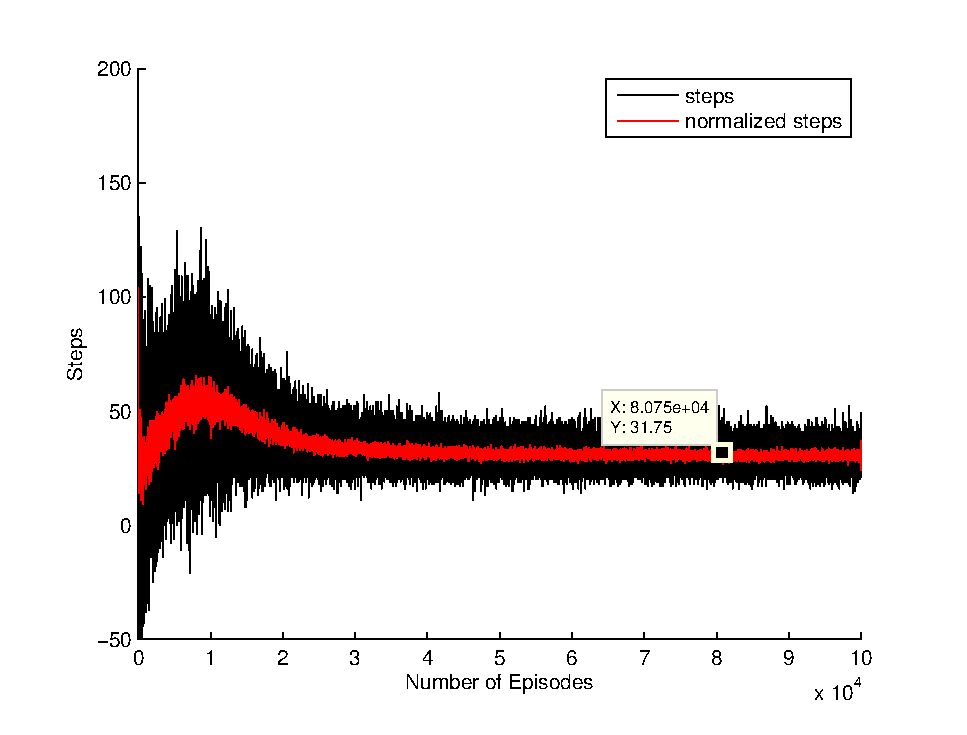
\includegraphics[width=0.7\textwidth]{figures/q207.eps}
    \caption{Performance of independent \textit{Q-Learning} algorithm, multi-agent environment (2 predators, 1 prey), $\alpha = 0.7$.}
    \label{q21}
\end{figure}
~
\begin{figure}[ht!]
  \centering
	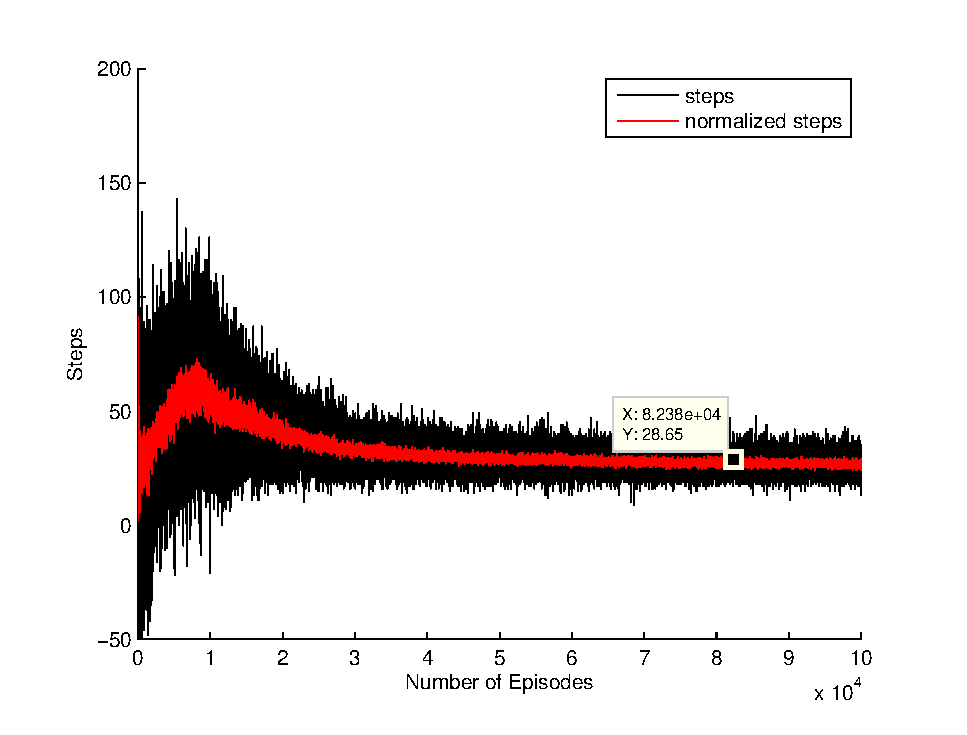
\includegraphics[width=0.7\textwidth]{figures/q205.eps}
   \caption{Performance of independent \textit{Q-Learning} algorithm, multi-agent environment (2 predators, 1 prey), $\alpha = 0.5$.}
    \label{q22}
\end{figure}
~
\begin{figure}[ht!]
  \centering
	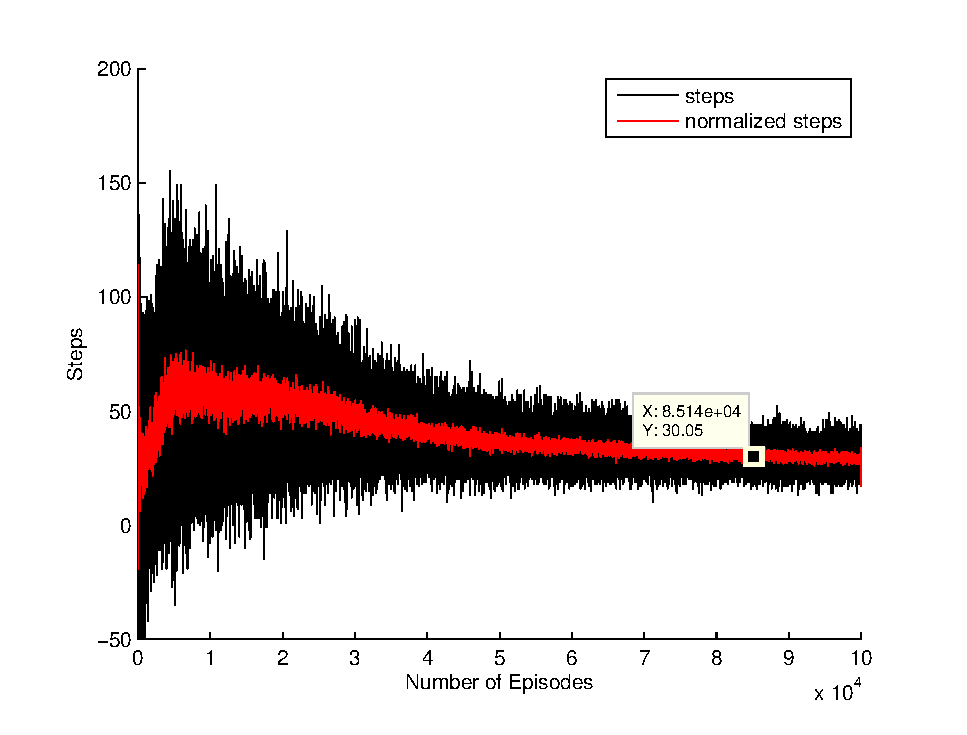
\includegraphics[width=0.7\textwidth]{figures/q202.eps}
    \caption{Performance of independent \textit{Q-Learning} algorithm, multi-agent environment (2 predators, 1 prey), $\alpha = 0.2$.}
    \label{q23}
\end{figure}

In this phase, we are going to illustrate through the following figures the performance that independent learning had in this multi-agent system. 
Figure~\ref{q21}, ~\ref{q22}, and, ~\ref{q23} illustrate our results in independent \textit{Q-Learning} with different values for learning rate, $\alpha = 0.7$, $\alpha = 0.5$, $\alpha = 0.2$, respectively. In addition, $\gamma$ parameter is always fixed at $0.7$, as we have seen it to perform really well for single agent {Q-Learning}. We can figure out that, as $\alpha$ is decreased, independent \textit{Q-Learning} needs more episodes to converge. All of the three versions converge almost at the same number of steps, indicating that an optimal policy has been found in all the three cases.   
One more interesting thing that these figures indicate, is the negative number of steps. Every time that there is a collision between the predators, we are saving the number of steps multiplied by $-1$ to be able to clearly illustrate their learning process. At the beginning of predators' learning we can see that, there is a random movement resulting in a big number of collisions between them. After one thousand episodes predators have learnt to avoid collisions and are focusing only on catching the prey as quick as possible. Lastly, the peak that appears in all figures indicates the end of the exploring phase (predators are still testing "bad" moves and paths), and the start of the exploiting phase, where predators have enough knowledge on how to avoid collisions and start chosing optimal paths towards the prey.

\begin{figure}[ht!]
  \centering
    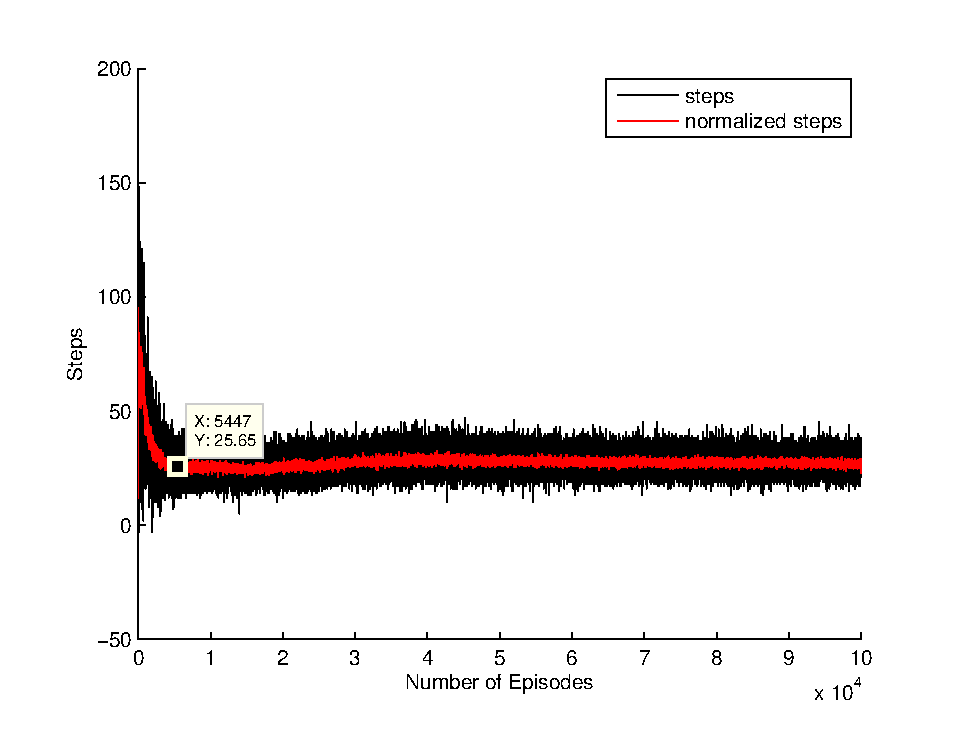
\includegraphics[width=0.49\textwidth]{figures/q2init.eps}\	
    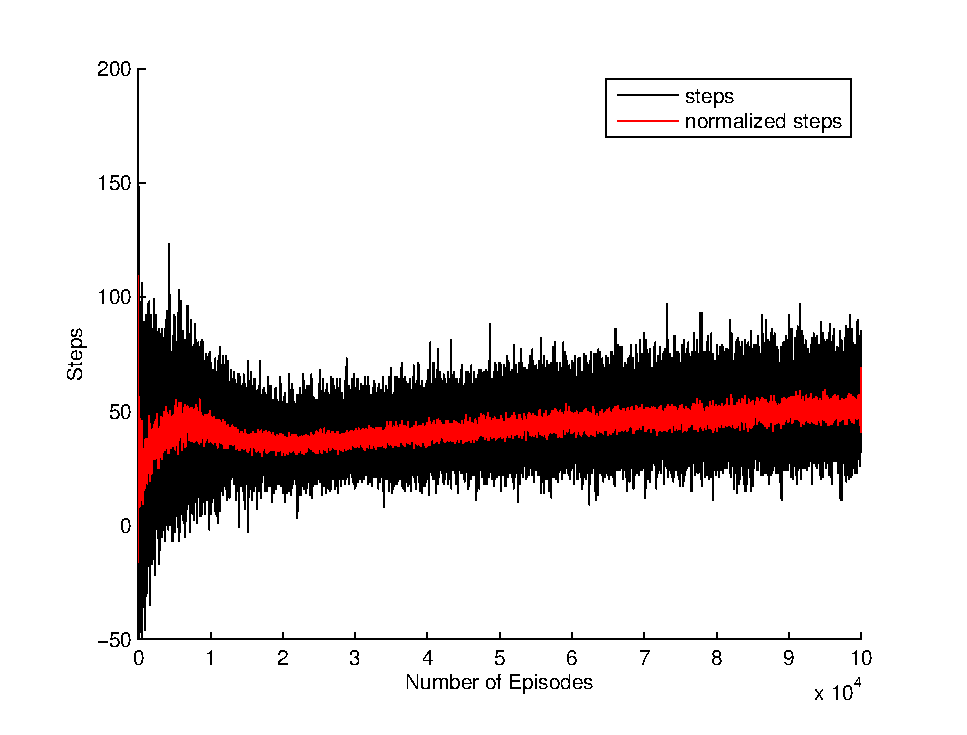
\includegraphics[width=0.49\textwidth]{figures/q2learnfast.eps}
    \caption{\textbf{Left:} Further testing of independent \textit{Q-Learning} algorithm, multi-agent environment (2 predators, 1 prey), $\alpha = 0.7$, Q-initialization to zero value. \textbf{Right:} Further testing of independent \textit{Q-Learning} algorithm, multi-agent environment (2 predators ($\alpha = 0.9$), 1 prey ($\alpha = 0.1$)).}
    \label{qtest}
\end{figure}

We also tried some changes in the parameters of the independent \textit{Q-Learning} algorithm in order to watch the agents' behavior under certain circumstances. Figure~\ref{qtest}, presents these two tests. In the first case, each agent initialized its Q-table with zero values (pessimistic). As we expected, the algorithm converged really fast, as the predators found an optimal policy fast enough without any need of further exploration. In the second case, predators' learning rate was significantly higher from the prey's. Predators learnt an optimal path really fast while the prey was still trying to improve its choices. We can see that after $1000$ episodes, the average number of steps increases continuously, indicating that the prey has at that moment started to find an optimal path aswell.


\subsection{Minimax Q-Learning}

In the second part of the first exercise we implemented the \textit{minimax Q-Learning} algorithm, as described in the paper: \textit{"Markov games as a framework for multi-agent reinforcement learning" by M.L. Littman, 1994}.

\subsubsection{Description}
First, the algorithm discussed in that paper is only described in a zero-sum two player Markov game. The obvious goal of both agents is to maximize their expected sum of discounted rewards, just like in an MDP. However, this algorithm discriminates the two agents by introducing a single reward function $R(s,a,o)$, which each agent tries to maximize and the other one (opponent) tries to minimize. So, for example, when the game is in state $s$, the predator will consider the prey choosing the optimal action $o$ which will minimize the expected reward of its opponent. As a consequence, the predator will choose the next possible action $s$ that maximizes its reward, always considering the worst case scenario. On the other hand, the prey will consider the predator picking the next possible action that is optimal. Generally, it is a fact that in the minimax-Q algorithm each agent considers its opponent to be optimal (picking the optimal actions each time), and defines its next action according to that. 

The \textit{minimax Q-Learning} algorithm consists of three parts: 	Initialization, choosing the next action and learning. Each agent initializes its own $Q[s,a,o]$ table, with initial value, $1$. For each possible state s, it also initializes the state value $V[s]$ table with initial value of $1$, as well. The probability between all the possible actions $a \in A$ deriving from each state $s$ is distributed equally, with $P(s,a_{i}) = 1/|A|$ $\forall a_i \in A$, and is also saved in the $\pi$-table, $pi[s,a]$. Learning rate $\alpha$ is also initialized as $1$ and will descend as the steps in each episode goes on. That means, the agents learn based on their immediate past in the beginning of the algorithm, but they consider their past to become more important in the next stages as they do not learn anymore if learning rate becomes very low.

After the initialization of the data, each agent will have to choose its next action. That depends on a variable $\epsilon$, so as, agents choose the action with maximum probability in the $pi[s,a]$ table with probability $1-\epsilon$, but they choose a random action among the possible ones with probability $\epsilon$. This is very similar to $\epsilon$-greedy action selection, but this time, the action is chosen based on its probability of being chosen and not on its expected reward. The learning part of the algorithm is described below:

\begin{itemize}
\item After receiving reward $R_t$ for moving from state $s$ to $s'$ , via action $a$ and opponent's action $o$,
\[
Q_{t+1}[s,a,o] = (1-\alpha)\times Q_t[s,a,o] + \alpha \times (r + \gamma \times V[s'])
\]

\item We used linear programming to find $pi[s,.]$ such that:
\[
pi[s,.] = \arg\max_{pi'[s,.]} {(\min_{o'} \sum_{a'} (pi[s,a'] \times Q[s,a',o']))}
\]
In fact we need to maximize what our opponent agent wants to minimize. The maximization term goes to the probabilities of choosing our set of actions, given that our opponent is going to minimize it. 

For the necessary linear programming part we used $6$ variables. One for the opponent's minimization $m$, and the remaining $5$ for our actions, $p_1$,$p_2$,\ldots,$p_5$. Linear programming needs constraints in order to maximize the given linear combination of variables. Our main function to maximize was $f(m)$, and the constraints were:
\begin{itemize}
\item $ \sum_{i}{p_i} = 1.0$
\item $ p_i \geq 0.0$
\item $ \sum_{a'} (pi[s,a'] \times Q[s,a',o']) \geq m$, $\forall o' \in O$
\end{itemize}
\item The value of the state s will be equal with the maximized value of variable from the linear program m: $V[s] = m$
\item Learning rate will be always decayed in each update: $\alpha = \alpha \times decay$. $decay \in (0,1)$ is the variable we use to reduce the value of $\alpha$.
\end{itemize}


\subsection{Results}

\begin{figure}[h]
\begin{center}
    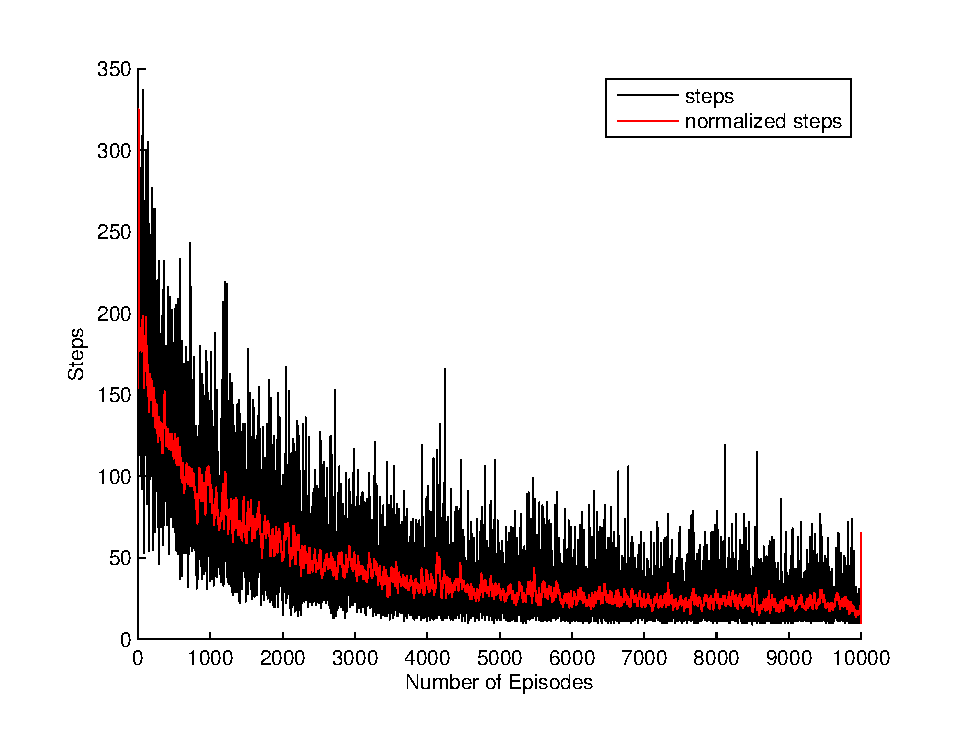
\includegraphics[width=0.7\textwidth]{figures/minimax0505.eps}
    \caption{Performance of  \textit{Minimax Q-Learning} algorithm, multi-agent environment (1 predator(\textit{Minimax Q-Learning}), 1 prey(random)), $\alpha = 0.5$, $\gamma = 0.5$.}
    \label{m11}
\end{center}
\end{figure}

\begin{figure}[h]
\begin{center}
	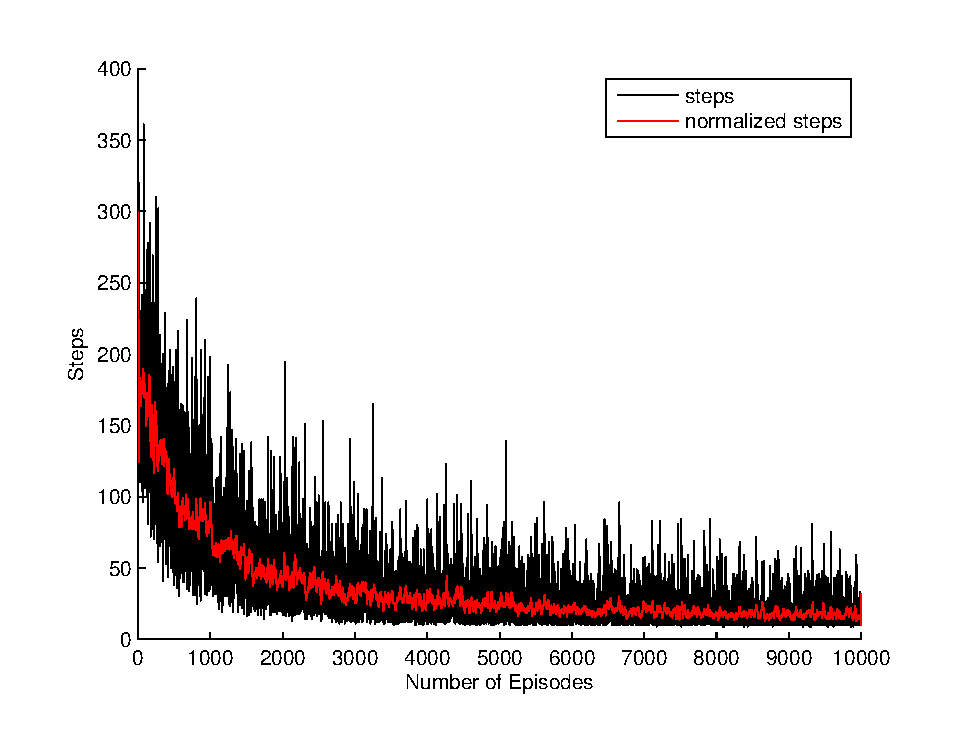
\includegraphics[width=0.7\textwidth]{figures/minimax0707.eps}
   \caption{Performance of  \textit{Minimax Q-Learning} algorithm, multi-agent environment (1 predator(\textit{Minimax Q-Learning}), 1 prey(random)), $\alpha = 0.7$, $\gamma = 0.7$.}
    \label{m22}
\end{center}
\end{figure}

\begin{figure}[h]
\begin{center}
    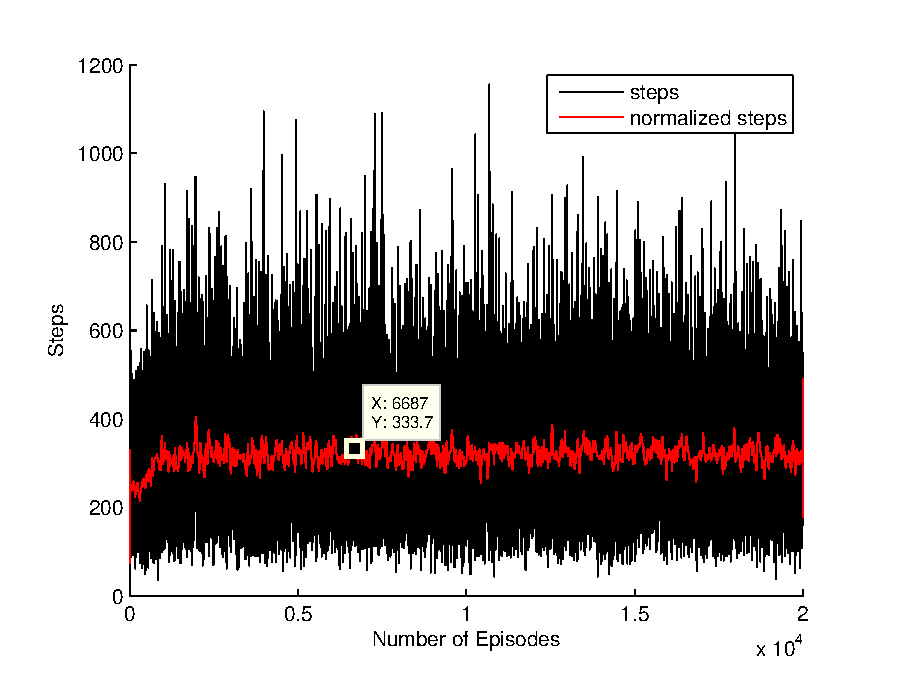
\includegraphics[width=0.49\textwidth]{figures/mm05.eps}\	
    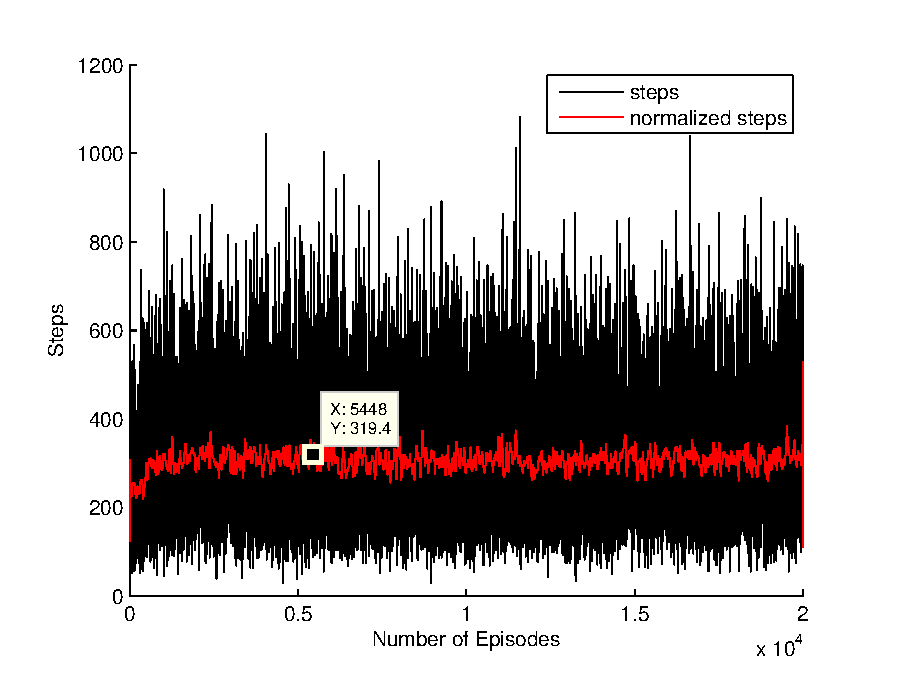
\includegraphics[width=0.49\textwidth]{figures/mm07.eps}\\
    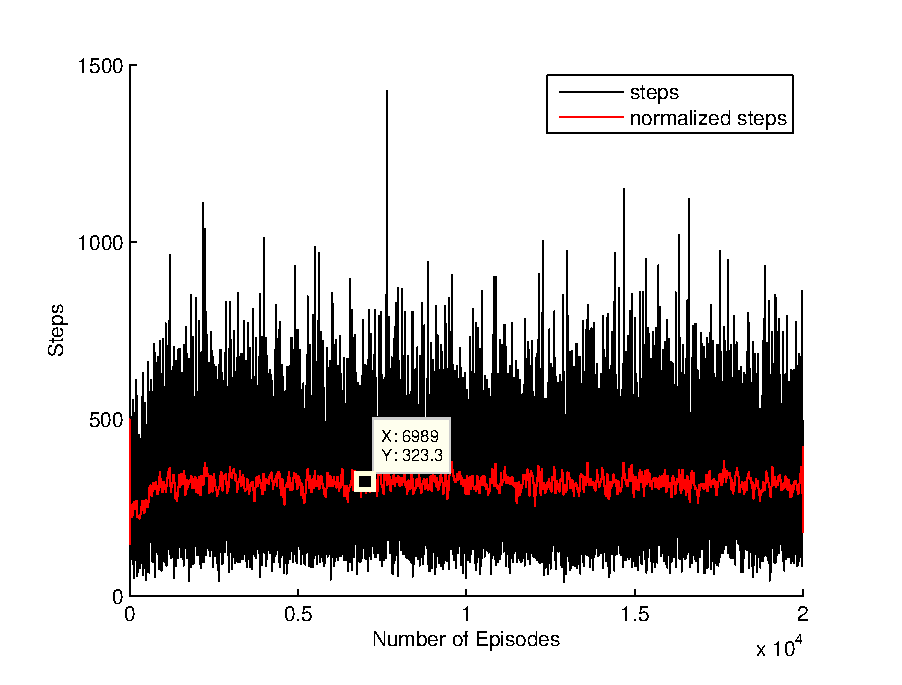
\includegraphics[width=0.5\textwidth]{figures/mm09.eps}
    \caption{Performance of  \textit{Minimax Q-Learning} algorithm, multi-agent environment (1 predator(\textit{Minimax Q-Learning}), 1 prey(\textit{Minimax Q-Learning})), \textbf{Left}: $\alpha = 0.5$, $\gamma = 0.7$, \textbf{Right}: $\alpha = 0.7$, $\gamma = 0.7$, \textbf{Middle}: $\alpha = 0.9$, $\gamma = 0.7$.}
    \label{m13}
\end{center}
\end{figure}

First, we wanted to test our implementation of the \textit{Minimax Q-learning} algorithm. We have done so by using predators which learn according to this method, and a prey with a random policy. Figure~\ref{m11} and Figure~\ref{m22}, shows the results we have in the approach with the random prey. We can see that, algorithm converges to a optimal policy for the predator. Although, we can see some peaks in the graph. The main characteristic of the \textit{Minimax Q-learning} is that we always consider our opponent to be optimal. This means that even predator was competing with a random prey, it was doing actions in respect that prey's best action. Therefore, we have a good reason why this is happening.

%!!!!!!!!!!!!!!!!!!!!!!!!!!!!!!!!!!!!!!!!!!!!!!!!!!!!!!!!!!!!!!!!!!!!
%here it is the part that we have to discuss why we have so fucking results
Next, we did the same but now both agents learn using the \textit{Minimax Q-learning} algorithm. Figure~\ref{m13},  presents our results in this part of the assignment. Although, we tested our implementation for possible bugs, we do not have a clear idea why it this thing happening. Algorithm does not seem to converge. Both agents use the policy that it is generated by the linear program in each update. Both agents use random actions with probability $p_{random} = 0.1$. The red line indicates that more than 300 steps is needed by the predator in average to catch the prey. This is not normal as the prey holds a probability to trip in every action that it takes.


\section{WoLF-PHC}
In the final part of the exercise we chose to implement \textit{Wolf-Policy Hill Climbing}. This algorithm is described in detail in the slides of the Autonomous Agents course. In addition, the paper \textit{``Efficient Learning in Games'', by Raghav Aras, Alain Dutech and Francois Charpillet}, was really useful for us in order to implement this algorithm.

The general idea behind this algorithm is that, agent chooses its action by its $\pi$-table in respect to the probability of each action. Next, agent updates its Q-table:
\[
Q_{t+1}(s,a) \leftarrow (1-\alpha)Q_{t}(s,a)+\alpha(r + \gamma \max_{a'}Q(s',a'))
\]
Next, agent has to update its average policy. Every state has a counter which indicated the times that was visited by the agent in the past. Using this counter, agent, is able to update the value of the its current state's policy for all actions:
\[
\bar{\pi}(s,b) \leftarrow \bar{\pi}(s,b) + \cfrac{1}{V} (\pi(s,b) - \bar{\pi}(s,b)), \forall b
\]
,where $V$ is the number of visits in this state. A big difference from the other learning algorithms is on the policy update. In general this algorithm uses two variables to change the probability of choosing the taken action. $\delta_{win}$, $\delta_{lose}$, the first one is used whenever agent chose an action which was better than the average policy and the second for the opposite case. This unique way to update the policy being followed by the agent is the main characteristic of this algorithm.


\subsection{Results}
Figures~\ref{w111}, ~\ref{w112}, ~\ref{w113}, and, ~\ref{w114}, present the results we have in \textit{WoLF-PHC} learning algorithm. We can see four different implementations with different parameters for $\delta$ variable. This parameter is the most important parameter of this algorithm. Through testing we realize that the performance of this algorithm depends heavily on the ratio: $\dfrac{\delta_{lose}}{\delta_{win}}$.

Then, we took the best parameters from the above experiments for, $\delta_{lose} = 0.3$, $\delta_{win} = 0.15$ and perform the same experiment for two predators, and one prey now. Figure~\ref{w2}, presents the results. \textit{WoLF-PHC}, converges to an average positive $50$ steps after two million episodes. So, it is clear that predators learn how not to collide with each other. Unfortunately, we were not able to perform the same test for more more episodes, but we believe that the learning process is depicted clear enough in this figure.

\subsubsection{Observations}
\begin{itemize}
\item In Figure~\ref{w111}, we used a ratio $\dfrac{\delta_{lose}}{\delta_{win}} = 2.5$. Fast converge of the algorithm in an average of $76$ steps.
\item In Figure~\ref{w112}, we used a ratio $\dfrac{\delta_{lose}}{\delta_{win}} = 2$. Slower converge than the first implementation , in an average of $54$ steps. Few random placed peaks up to 300 steps.
\item In Figure~\ref{w113}, we used a ratio $\dfrac{\delta_{lose}}{\delta_{win}} = 3$. Slower converge than the first two implementations, in an average of $35$ steps. More random placed peaks up to 900 steps.
\item In Figure~\ref{w114}, we used a ratio $\dfrac{\delta_{lose}}{\delta_{win}} = 5$. Same converge with the previous implementation, in an average of $39$ steps. Lots of random placed peaks up to 3000 steps (Are not shown in the figure due to scale equality of the four figures).
\end{itemize}

The first thing we want to mention is that, the converge speed of this learning algorithm is mainly depends on how big values we used for $\delta_{win}$. As $\delta_{win}$ went down, algorithm converged in a better average of steps. This happened because for every visited state is giving agent just adds a small value in the best policy causing the same effect $\alpha$ parameter has in pure \textit{Q-Learning}.

Second, we have noticed an increasing number of peaks as the ratio $\dfrac{\delta_{lose}}{\delta_{win}}$ is going up. A big ratio means that, agents are able to perform huge changes in their policies as $\delta_{lose}$ is now a lot bigger than the $\delta_{win}$. For example, prey is always ``disappointed'' from its policy and tries to change it causing these abnormal peaks.

\begin{figure}[ht!]
  \centering
    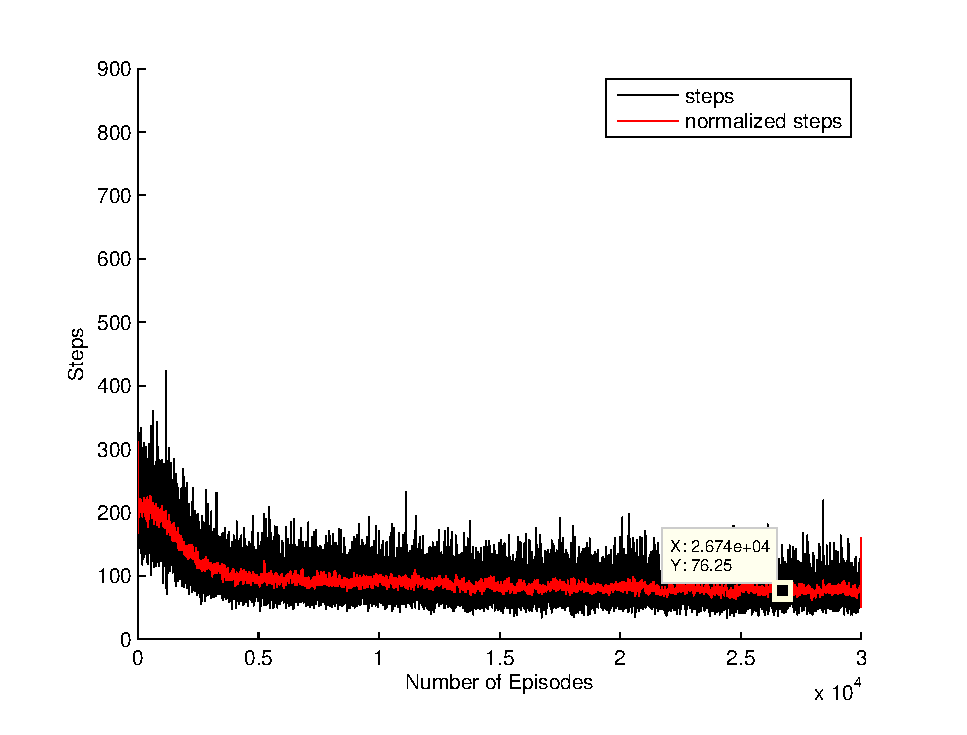
\includegraphics[width=0.7\textwidth]{figures/w07070502.eps}
    \caption{Performance of  \textit{WoLF-PHC} algorithm, multi-agent environment (1 predator(\textit{WoLF-PHC}), 1 prey(\textit{WoLF-PHC})), $\alpha = 0.7$, $\gamma = 0.7$, $\delta_{lose} = 0.5$, $\delta_{win} = 0.2$.}
    \label{w111}
\end{figure}
~
\begin{figure}[ht!]
  \centering
    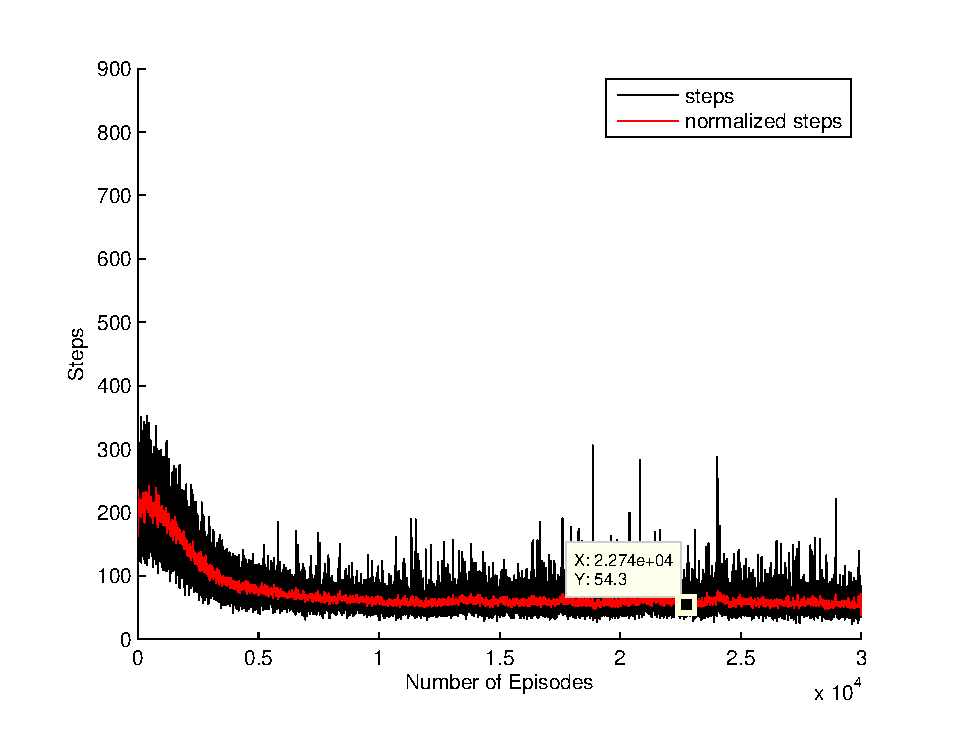
\includegraphics[width=0.7\textwidth]{figures/w070703015.eps}
       \caption{Performance of  \textit{WoLF-PHC} algorithm, multi-agent environment (1 predator(\textit{WoLF-PHC}), 1 prey(\textit{WoLF-PHC})), $\alpha = 0.7$, $\gamma = 0.7$, $\delta_{lose} = 0.3$, $\delta_{win} = 0.15$.}
    \label{w112}
\end{figure}
~
\begin{figure}[ht!]
  \centering
    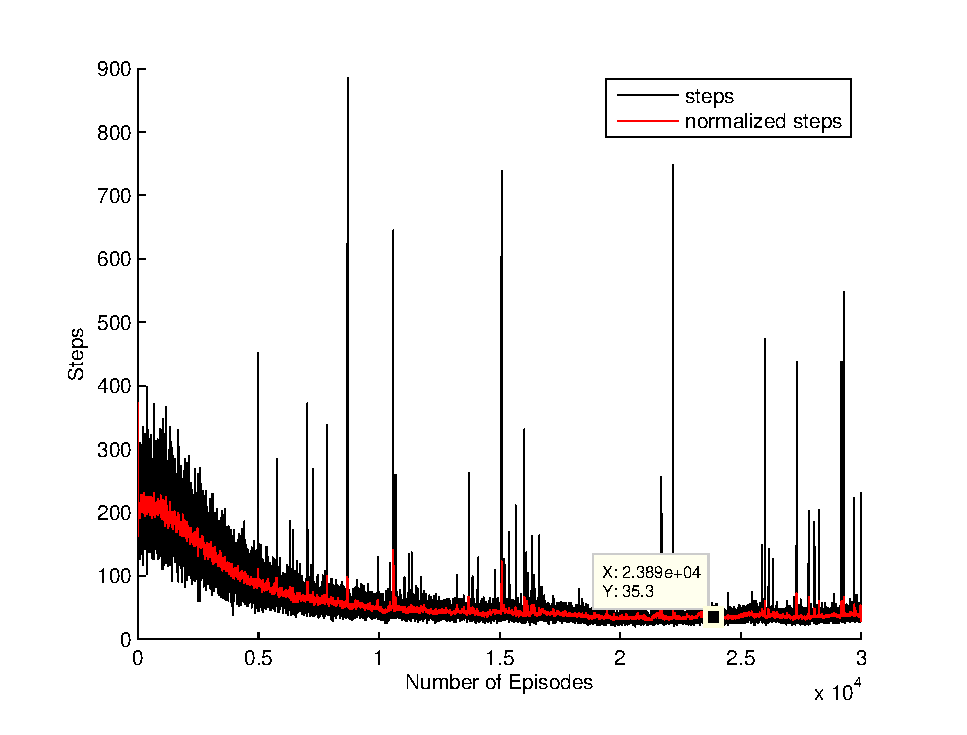
\includegraphics[width=0.7\textwidth]{figures/w0707015005.eps}
        \caption{Performance of  \textit{WoLF-PHC} algorithm, multi-agent environment (1 predator(\textit{WoLF-PHC}), 1 prey(\textit{WoLF-PHC})), $\alpha = 0.7$, $\gamma = 0.7$, $\delta_{lose} = 0.15$, $\delta_{win} = 0.05$.}
    \label{w113}
\end{figure}
~
\begin{figure}[ht!]
  \centering
    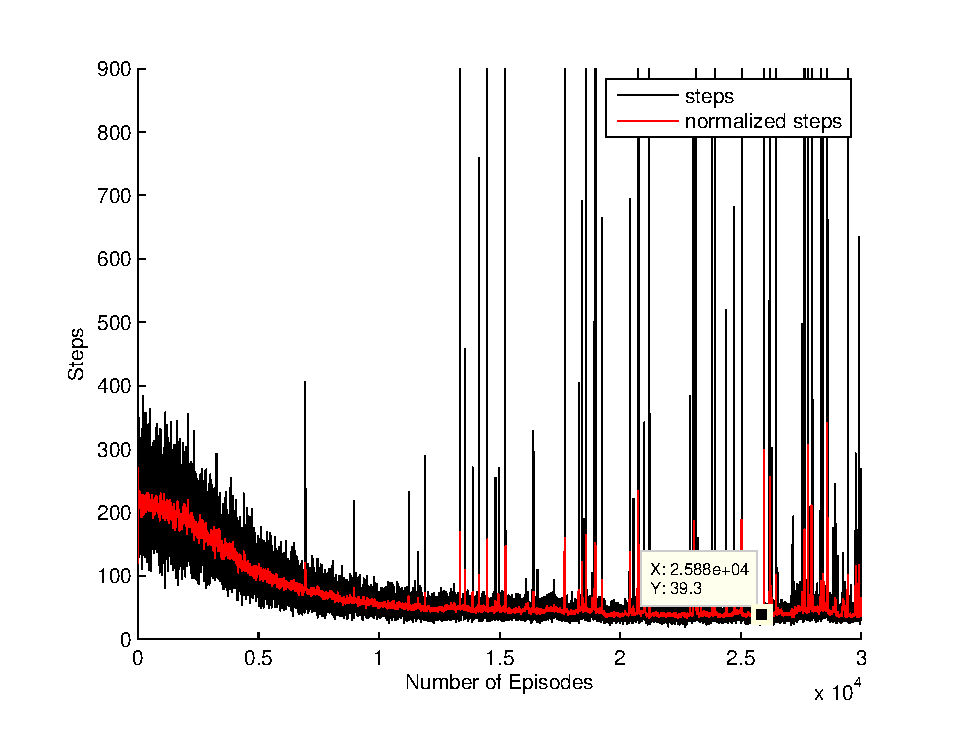
\includegraphics[width=0.7\textwidth]{figures/w070701002.eps}
        \caption{Performance of  \textit{WoLF-PHC} algorithm, multi-agent environment (1 predator(\textit{WoLF-PHC}), 1 prey(\textit{WoLF-PHC})), $\alpha = 0.7$, $\gamma = 0.7$, $\delta_{lose} = 0.1$, $\delta_{win} = 0.02$.}
    \label{w114}
\end{figure}
~
\begin{figure}[ht!]
  \centering
    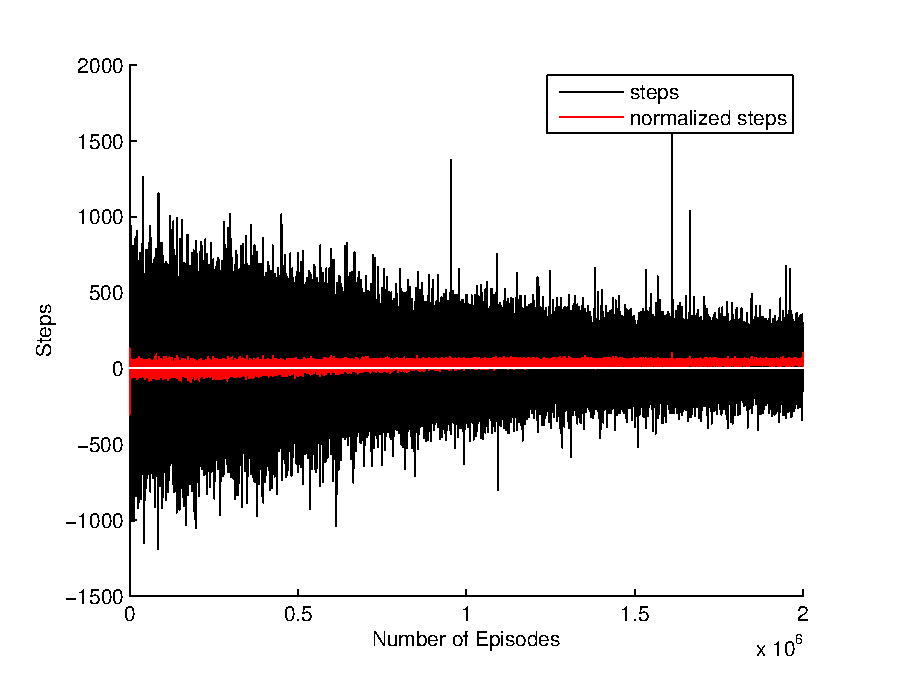
\includegraphics[width=0.9\textwidth]{figures/w2.eps}
        \caption{Performance of  \textit{WoLF-PHC} algorithm, multi-agent environment (2 predator(\textit{WoLF-PHC}), 1 prey(\textit{WoLF-PHC})), $\alpha = 0.7$, $\gamma = 0.7$, $\delta_{lose} = 0.3$, $\delta_{win} = 0.15$.}
    \label{w2}
\end{figure}

\newpage

\section{Conclusion}
In this last assignment of the Autonomous Agents course, we implemented and experimented on different learning algorithms that can be used in multi-agent frameworks. We comprehend how more than one agents can explode the space complexity of these specific algorithms, considering that fact, we can understand the reason why planning and learning in multi-agent system have triggered a great research interest the last decade.

\end{document}